\documentclass{standalone}
\usepackage{tikz}
\usepackage{pgfmath}
\usetikzlibrary{positioning}
\usetikzlibrary{calc}

\begin{document}
    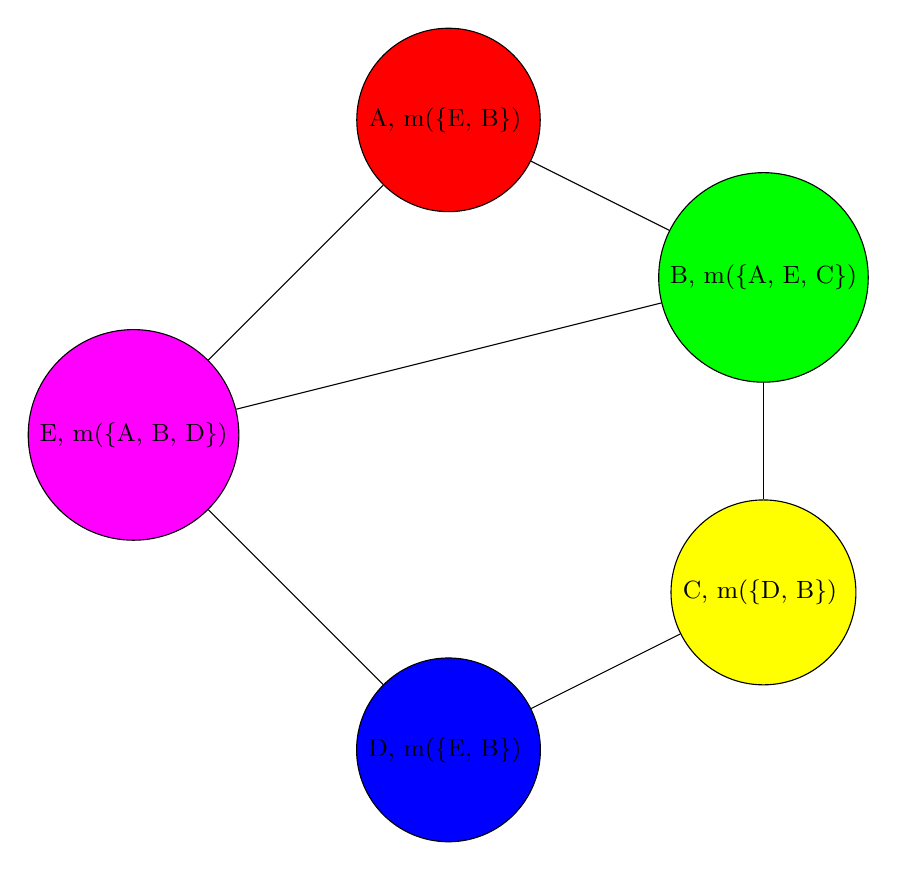
\begin{tikzpicture}[
        scale=1, 
        every node/.style={circle, draw, minimum size=2cm},
    ]
        % Color palette
        \definecolor{attr1}{RGB}{255,0,0}
        \definecolor{attr2}{RGB}{0,255,0}
        \definecolor{attr3}{RGB}{255,255,0}
        \definecolor{attr4}{RGB}{0,0,255}
        \definecolor{attr5}{RGB}{255,0,255}
        % Initial State
        % Message Aggregation State
        \node[fill=attr1] (A) at (0,4) {\small {A, m(\{E, B\})\;}};
        \node[fill=attr2] (B) at (4,2) {\small {B, m(\{A, E, C\})}};
        \node[fill=attr3] (C) at (4,-2) {\small {C, m(\{D, B\})\;}};
        \node[fill=attr4] (D) at (0,-4) {\small {D, m(\{E, B\})\;}};
        \node[fill=attr5] (E) at (-4,0) {\small {E, m(\{A, B, D\})}};

        % Edges
        \draw (A) -- (B);
        \draw (A) -- (E);
        \draw (B) -- (C);
        \draw (C) -- (D);
        \draw (D) -- (E);
        \draw (B) -- (E);

    \end{tikzpicture}

\end{document}